\documentclass[12pt, letterpaper, twoside]{article}
\usepackage[utf8]{inputenc}
\usepackage[spanish]{babel}
\usepackage{amsmath, amsfonts, amssymb, amsthm}
\usepackage[left = 2cm, right = 2cm, top = 2cm, bottom = 2cm]{geometry}

\title{Grafos}

%Estilo de la página
\usepackage{fancybox, fancyhdr}
\pagestyle{fancy}
\fancyhf{}
\fancyhead[LE,RO]{\small{\leftmark}}
\fancyfoot[CE,CO]{\thepage}
\renewcommand{\headrulewidth}{2 pt}

%Imagenes
\usepackage{graphicx}
\graphicspath{{Imagenes/}}

%Estilo del codigo
\usepackage{listings}
\usepackage[dvipsnames]{xcolor}
\lstset{  
	language         = C++, 
	xleftmargin      = 1 cm,
	numbers          = left,
	numberstyle      = \tiny\textbf,	
	basicstyle       = \footnotesize,
	keywordstyle     = \color{blue},
	directivestyle   = \color{Green},
	commentstyle     = \color{purple},
	stringstyle      = \color{blue},
	showstringspaces = false,
	breaklines       = true,
	%emph             = {std, cin, cout, min, max, swap, vector, queue},   
	emphstyle        = \color{Green},
}

%Documento
\begin{document}

\section{Máximo flujo.}

Consideremos un grafo dirigido $G = (V, E)$ donde cada arista $(u, v)$ tiene asociada una capacidad $c(u,v) > 0$. Un flujo de $s$ a $t$ es una función que a cada arista le asigna un número $f(u,v)$ que satisface
\begin{itemize}
\item $f(u, v) \leq c(u,v)$.
\item Para cualquier vértice $v \neq s, t$, el flujo que entra es igual al flujo que sale; $s$ solo tiene flujo saliente y $t$ solo tiene flujo entrante.
\end{itemize}
El flujo total es el flujo que sale de $s$.

\begin{center}
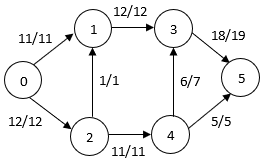
\includegraphics[width = 0.4\textwidth]{MaxFlow.png}	
\end{center}

\subsection{Algoritmo de Edmonds-Karp}

Complejidad: $O(\min\{|V||E|^2, |E| \max f\})$.

\lstinputlisting[firstline = 6]{Edmonds-Karp.cpp} 

\begin{tabular}{|p{7cm}|p{7cm}|}
\hline
\textbf{Entrada} & \textbf{Salida}\\ \hline
6 8 & Flujo maximo: 23\\
0 1 11 & 0 1: 11/11\\
0 2 12 & 0 2: 12/12\\
1 3 12 & 1 3: 12/12\\
2 1 1  & 2 1: 1/1\\
2 4 11 & 2 4: 11/11\\
4 3 7  & 3 5: 18/19\\
3 5 19 & 4 3: 6/7\\
4 5 5 & 4 5: 5/5\\ \hline
\end{tabular}

\end{document}